\documentclass{bmstu}

\bibliography{biblio}
\usepackage{svg}
\usepackage{algpseudocode}
\usepackage{longtable}
\usepackage{listings}

\definecolor{darkgray}{gray}{0.15}

\lstset{
	language=python, % выбор языка для подсветки
	basicstyle=\small\sffamily, % размер и начертание шрифта для подсветки кода
	numbers=left, % где поставить нумерацию строк (слева\справа)
	%numberstyle=, % размер шрифта для номеров строк
	stepnumber=1, % размер шага между двумя номерами строк
	numbersep=5pt, % как далеко отстоят номера строк от подсвечиваемого кода
	frame=single, % рисовать рамку вокруг кода
	tabsize=2, % размер табуляции по умолчанию равен 4 пробелам
	captionpos=t, % позиция заголовка вверху [t] или внизу [b]
	breaklines=true,
	breakatwhitespace=true, % переносить строки только если есть пробел
	backgroundcolor=\color{white},
	keywordstyle=\color{blue}
}

\begin{document}

\setlist[enumerate]{label=\arabic*)}
\setlist[itemize]{label=---}

\makereporttitle{Информатика и системы управления}
{Программное обеспечение ЭВМ и информационные технологии}
{лабораторной работе № 6}
{Анализ Алгоритмов}
{Методы решения задачи коммивояжёра}
{}{А. А. Кузин/ИУ7-51Б}{Л. Л. Волкова}


\renewcommand{\contentsname}{Содержание}
\tableofcontents
\setcounter{page}{2}
\chapter*{ВВЕДЕНИЕ}
\addcontentsline{toc}{chapter}{ВВЕДЕНИЕ}

Цель лабораторной работы -- реализация методов решения задачи коммивояжера на основе муравьиного алгоритма.

Задачи данной лабораторной:
\begin{itemize}
	\item описать задачу коммивояжера;
	\item описать методы решения задачи коммивояжера --- метод полного перебора и метод на основе муравьиного алгоритма;
	\item реализовать выбранные алгоритмы;
	\item провести функциональное тестирование разработанных алгоритмов;
	\item исследовать время работы реализаций алгоритмов.  
\end{itemize}

\chapter{Аналитическая часть}
В этом разделе будут рассмотрена информация, касающаяся задачи коммивояжера, а также способы их решения.


\section{Задача коммивояжера}

Задача коммивояжёра \text{(англ. \textit{traveling salesman problem})} --- (задача о бродячем торговце) одна из самых важных задач всей транспортной логистики, в которой рассматриваются вершины графа, а также матрица смежности (для расстояния между вершинами)\,\cite{task}. 
Задача заключается в том, чтобы найти такой порядок посещения вершин графа, при котором путь будет минимален, каждая вершина будет посещена лишь один раз, а возврат произойдет в начальную вершину. 



\section{Метод полного перебора для решения задачи коммивояжёра}

Полный перебор для задачи коммивояжёра~\cite{fullcomb} имеет высокую сложность алгоритма ($n!$), где $n$ --- количество городов. 
Суть в полном переборе всех возможных путей в графе и выбор наименьшего из них. 
Решение будет получено, но имеются большие затраты по времени выполнения при уже небольшом количестве вершин в графе.

\section{Метод на основе муравьиного алгоритма}

Муравьиный алгоритм (англ. \textit{ant colony optimization}) \cite{fullcomb} --- метод решения задачи оптимизации, основаный на принципе поведения колонии муравьев.

Муравьи действуют, руководствуясь органами чувств. 
Каждый муравей оставляет на своём пути феромоны, чтобы другие могли ориентироваться. 
При большом количестве муравьев наибольшее количество феромона остаётся на наиболее посещаемом пути, посещаемость же может быть связана с длинами рёбер.

Суть в том, что отдельно взятый муравей мало что может, поскольку он способен выполнять только максимально простые задачи. Но при большом числе других таких муравьев они могут выступать самостоятельными вычислительными единицами. Муравьи используют непрямой обмен информацией через окружающую среду посредством феромона.


Пусть муравей имеет следующие характеристики:
\begin{enumerate}[label=\arabic*.]
	\item зрение --- способность определить длину ребра;
	\item память --- способность запомнить пройденный маршрут;
	\item обоняние --- способность чуять феромон.
\end{enumerate}


Также введем целевую функцию \eqref{d_func}, характеризующую привлекательность ребра, определяемую благодаря зрению.

\begin{equation}
	\label{d_func}
	\eta_{ij} = 1 / D_{ij},
\end{equation}
где $D_{ij}$ — расстояние от текущего пункта $i$ до заданного пункта $j$.


Также понадобится формула вычисления вероятности перехода в заданную точку \eqref{posib}.

\begin{equation}
	\label{posib}
	p_{k,ij} = \begin{cases}
		\frac{\eta_{ij}^{\alpha}\cdot\tau_{ij}^{\beta}}{\sum_{q\notin J_k} \eta^\alpha_{iq}\cdot\tau^\beta_{iq}}, j \notin J_k \\
		0, j \in J_k
	\end{cases}
\end{equation}
где $a$ --- параметр влияния длины пути, $b$ --- параметр влияния феромона, $\tau_{ij}$ --- количество феромонов на ребре $ij$, $\eta_{ij}$ --- привлекательность ребра $ij$, $J_k$ --- список посещённых за текущий день городов.

После завершения движения всех муравьев (ночью, перед наступлением следующего дня), феромон обновляется по формуле \eqref{update_phero_1}.
\begin{equation}
	\label{update_phero_1}
	\tau_{ij}(t+1) = \tau_{ij}(t)\cdot(1-p) + \Delta \tau_{ij}(t).
\end{equation}
При этом
\begin{equation}
	\label{update_phero_2}
	\Delta \tau_{ij}(t) = \sum_{k=1}^N \Delta \tau^k_{ij}(t),
\end{equation}
где
\begin{equation}
	\label{update_phero_3}
	\Delta\tau^k_{ij}(t) = \begin{cases}
		Q/L_{k}, \textrm{ребро посещено муравьем $k$ в текущий день $t$,} \\
		0, \textrm{иначе}
	\end{cases}
\end{equation}

Поскольку вероятность перехода в заданную точку \ref{posib} не должна быть равна нулю, необходимо обеспечить неравенство $\tau_{ij} (t)$ нулю посредством введения дополительного минимально возможного значения феромона $\tau_{min}$ и в случае, если $\tau_{ij} (t+1)$ принимает значение, меньшее $\tau_{min}$, откатывать феромон до этой величины. 


Путь выбирается по следующей схеме.
\begin{enumerate}
	\item Каждый муравей имеет список запретов --- список уже посещенных городов (вершин графа).
	\item Муравьиное зрение отвечает за эвристическое желание посетить вершину.
	\item Муравьиное обоняние отвечает за ощущение феромона на определенном пути (ребре). При этом количество феромона на пути (ребре) в день $t$ обозначается как $\tau_{i, j} (t)$.
	\item После прохождения определенного ребра муравей откладывает на нем некотрое количество феромона, которое показывает оптимальность сделанного выбора, это количество вычисляется по формуле \eqref{update_phero_3}.
\end{enumerate}

% \addcontentsline{toc}{section}{Вывод}
\section*{Вывод}
В этом разделе была рассмотрена задача коммивояжёра, а также полный перебор для её решения и муравьиный алгоритм.
\clearpage

\chapter{Конструкторская часть}

В этом разделе будут представлено описание используемых типов данных, а также псевдокод алгоритма поиска в словаре.

К программе предъявлен ряд функциональных требований:
\begin{itemize}
	\item иметь интерфейс ввода вопроса;
	\item работа с словарями и строками;
\end{itemize}

\section{Описание используемых типов данных}
При реализации алгоритмов будут использован словрь --- встроенный тип dict в Python:
\section{Разработка алгоритмов}

В листинге\ref{lst:alg1} представлен псевдокод алгоритма поиска в словаре полным перебором.

% \includeimage
% {full_comb} % Имя файла без расширения (файл должен быть расположен в директории inc/img/)
% {f} % Обтекание (без обтекания)
% {H} % Положение рисунка (см. figure из пакета float)
% {1\textwidth} % Ширина рисунка
% {Схема алгоритма поиска в словаре полным перебором} % Подпись рисунка

\begin{lstlisting}[breakatwhitespace=false, label=lst:alg1, caption=Алгоритм поиска в словаре полным перебором]
	input: dictionary dict, string key
   output: value
   
   for each dict.key
   begin
	if dict[key] = key then
	begin
		return dict[key].value
	end
   end
   return "no string found"
   \end{lstlisting}

\section*{Вывод}
% \addcontentsline{toc}{section}{Вывод}

В данном разделе были представлены требования к программе, представлен псевдокод алгоритма поиска значения в словаре.

\clearpage
\chapter{Технологическая часть}
В данном разделе будут приведены средства реализации, листинг кода и функциональные тесты.

\section{Средства реализации}

В качестве языка программирования, используемого при написании данной лабораторной работы, был выбран C++ \cite{cpp-lang}. Для замеров времени выбрана библиотека \texttt{<ctime>} \cite{ctime}, позволяющая производить замеры процессорного времени.

В качестве среды для написания кода был выбран \textit{Visual Studio Code} за счет того, что она предоставляет функционал для проектирования, разработки и отладки ПО.

\section{Сведения о модулях программы}

Данная программа разбита на следующие модули:

\begin{itemize}
    \item \texttt{main.cpp}~--- точка входа программы, пользовательское меню;
    \item \texttt{general}~--- модуль с основными конвеерными операциями;
    \item \texttt{csr\_matrix}~--- модуль с реализациями алгоритмов работы над матрицами;
    \item \texttt{measurement}~--- модуль с реализацией функции подсчета затрачиваемого времени.
\end{itemize}



\clearpage

\section{Реализация алгоритмов}

Далее будут представлены реализация для линейного и конвейерного алгоритмов обработки матриц. Также представлена реализация запуска 1, 2 и 3 потоков.


\includelistingpretty
    {general.cpp}
    {c}
    {Реализация конвеерных алгоритмов}
	
\clearpage

\section{Функциональные тесты}

В данном разделе будут представлены функциональные тесты, проверяющие работу алгоритмов сортировок.

В таблице \ref{tbl:func_test} приведены тесты для функций, реализующих алгоритмы сортировок.

\begin{table}[h!]
	\begin{center}
		\caption{\label{tbl:func_test}Тестирование функций}
		\begin{tabular}{|c|c|c|c|}
			\hline
			\textbf{Алгоритм} & \textbf{Кол-во матриц} & \textbf{Размер матриц} & \textbf{Результат} \\ 
			\hline
			Конвейерная & -1  & 10 & Ошибка \\\hline
			Конвейерная & 10  & -1 & Ошибка \\\hline
			Линейная & 10  & 5 & Вывод результата \\\hline
			Конвейерная & 10  & 10 & Вывод результата \\\hline
		\end{tabular}
	\end{center}
\end{table}

% \addcontentsline{toc}{section}{Вывод}
\section*{Вывод}
Были выбраны язык программирования и среда разработки, приведены сведения о модулях программы, листинги алгоритма, проведено функциональное тестирование.
\chapter{Исследовательская часть}

\section{Технические характеристики}
Технические характеристики устройства, на котором выполнялись
замеры по времени:

\begin{itemize}
    \item Процессор: Intel Core i7 9750H 2.6 ГГц;
    \item Оперативная память: 16 ГБ;
    \item Операционная система: Kubuntu 22.04.3 LTS x86\_64 Kernel: 6.2.0-36-generic
\end{itemize}

Во время проведения измерений времени ноутбук был подключен к сети электропитания и был нагружен только системными приложениями.

\section{Демонстрация работы программы}

На рисунке \ref{fig:img_prog} показан пример работы с программой.


\begin{figure}[ht!]
	\centering
	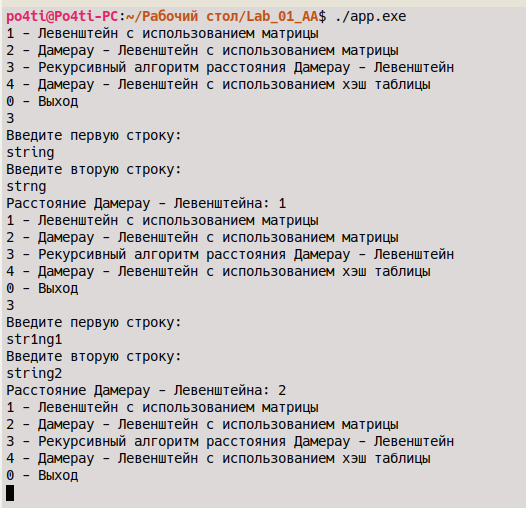
\includegraphics[width=170mm]{img/img_prog.png}
	\caption{Демонстрация работы программы.\label{overflow}}
	\label{fig:img_prog}
	\end{figure}


\clearpage

\section{Временные характеристики}


Исследование временных характеристик реализованных алгоритмов производилось на массивах размером 1 -- 500 с шагом 10.

\begin{figure}[ht!]
	\centering
	\includesvg[width=1.0\textwidth]{img/plotting_data1.svg}
	\caption{Результат измерений времени работы (в мс) алгоритмов сортировок на неотсортированных массивах\label{overflow}}
	\label{fig:plotting_data1}
	\end{figure}
\clearpage

\begin{figure}[ht!]
	\centering
	\includesvg[width=1.0\textwidth]{img/plotting_data2.svg}
	\caption{Результат измерений времени работы (в мс) алгоритмов сортировок на отсортированных массивах\label{overflow}}
	\label{fig:plotting_data2}
	\end{figure}

\begin{figure}[ht!]
	\centering
	\includesvg[width=1.0\textwidth]{img/plotting_data3.svg}
	\caption{Результат измерений времени работы (в мс) алгоритмов сортировок на отсортированных обратно массивах\label{overflow}}
	\label{fig:plotting_data3}
	\end{figure}

	
\section{Характеристики по памяти}

Пусть дан массив N элементов сравниваемого типа int. Тогда затраты по памяти для алгоритмов будут следующие:

\subsection*{Плавная сортировка}

Используемые переменные:
\begin{itemize}
	\item k первых чисел леонардо -- $k \cdot size(int)$
	\item переменные i, j, k в heapify -- $3 \cdot size(int)$
	\item переменные p q r в теле алгоритма -- $3 \cdot size(int)$
	\item массив -- $N \cdot size(int)$
	\item переменная-буфер для обмена элементов местами -- $1 \cdot size(int)$
\end{itemize}

Итого, для плавной сортировки:
\begin{equation}
M_{smooth} = k \cdot size(int) + 3 \cdot size(int) + 3 \cdot size(int) + N \cdot size(int) + 1 \cdot size
\end{equation}

\begin{equation}
M_{smooth} = (k + N + 7) \cdot size(int)	
\end{equation}

\subsection*{Сортировка перемешиванием}

Используемые переменные:
\begin{itemize}
	\item переменные right, left -- $2 \cdot size(int)$
	\item массив -- $N \cdot size(int)$
	\item переменная-буфер для обмена элементов местами -- $1 \cdot size(int)$
\end{itemize}

Итого, для сортировки перемешиванием:
\begin{equation}
M_{shake} = 2 \cdot size(int) + N \cdot size(int) + 1 \cdot size = (3 + N) \cdot size(int)	
\end{equation}

\subsection*{Сортировка Шелла}

Используемые переменные:
\begin{itemize}
	\item переменные right, left, gap -- $3 \cdot size(int)$
	\item массив -- $N \cdot size(int)$
	\item переменная-буфер для обмена элементов местами -- $1 \cdot size(int)$
\end{itemize}

Итого, для сортировки Шелла:
\begin{equation}
M_{shell} = 3 \cdot size(int) + N \cdot size(int) + 1 \cdot size = (4 + N) \cdot size(int)	
\end{equation}

\addcontentsline{toc}{section}{Вывод}
\section*{Вывод}

Самым быстрым алгоритмом на неотсортированных массивах является сортировка Шелла. Самым медленным - сортировка перемешиванием.

На отсортированных массивах сортировка Шелла и плавная сортировка имеют одинаковую асимптотику и являются самыми быстрыми.

При отсортированных в обратном порядке массивах самым быстрым алгоритмом является сортировка Шелла, самым медленным - плавная сортировка.

Самым эффективным алгоритмом по затраченному объему памяти является сортировка перемешиванием. Наименее эффективным ~-- плавная сортировка. 
\chapter*{ЗАКЛЮЧЕНИЕ}
\addcontentsline{toc}{chapter}{ЗАКЛЮЧЕНИЕ}

В ходе лабораторной работы поставленная ранее цель была достигнута:
были изучены принципы поиска по обычному и сегментированному словарю. 

В среднем, использование сегментированного словаря занимает меньше времени, чем использование обычного словаря. Особенно, если ключ ближе к последнему сегменту, выгода от использования сегментированного словаря увеличивается в 1.5 раза. Однако, если поиск направлен к первому сегменту, выполнение поиска в обычном словаре становится более выгодным.

В ходе выполнения лабораторной работы были решены следующие задачи:

\begin{enumerate}
    \item изучены алгоритмы поиска в словарях;
    \item описаны алгоритмы в виде псевдокода;
    \item реализованы алгоритмы поиска значения по ключу в стандартном и сегментированном словарях;
    \item проведен сравнительный анализ алгоритма поиска в стандартном и сегментированном словарях;
    \item описаны и обоснованы полученные результаты.
\end{enumerate}


\makebibliography

\end{document}